\documentclass[11pt]{scrartcl}
\usepackage{graphicx}
\usepackage{indentfirst}
\usepackage[most]{tcolorbox}
\usepackage{xcolor}
\usepackage{asymptote}
\usepackage{subfigure}

\definecolor{vocabcolor}{RGB}{175, 118, 196}

\title{Burnside Lemma}
\author{\LARGE Aatmik Krishna }
\date{\large March 2025}

\begin{document}
\maketitle

\section{Preface}
\large

In this handout, we will demonstrate the method of the Burnside Lemma. This will be done in an example-problem fashion, where we will give some example problems to demonstrate, then give you exercises and problems. 

\section{Introduction}

The \color{blue} \textbf{Burnside Lemma} \color{black} is a method of solving \textit{combinatorics} problems which have some kind of \textbf{symmetry} involved in them.

\begin{tcolorbox}[colback=orange!5!white,colframe=orange!75!black]
  Examples of when to \textbf{use} it:
  \begin{itemize}
  \item Problems where \color{blue} \textbf{rotations and/or reflections are considered equivalent}\color{black}.
  \begin{itemize}
      \item How many ways are there to color the sides of a square $2$ colors, where \textbf{rotations and reflections are considered equivalent}?
      \item How many ways can you arrange 4 distinct keys on a rings such that \textbf{rotations and reflections are considered equivalent}?
  \end{itemize}
  \item Problems where \color{blue} \textbf{symmetry causes overcounting}\color{black}.
  \end{itemize}
  Examples of when \textbf{not} to use it:
  \begin{itemize}
      \item When there are \textbf{many} symmetries.
      \item When there \textbf{isn't a clear connection} between configurations that shows some kind of symmetry.
  \end{itemize}
\end{tcolorbox}

As you can see, the entire method is based on solving problems to do with \color{blue} \textbf{symmetry}\color{black}. However, later on, we will see that many problems that have no apparent connection to the lemma can in fact be solved by it. \textit{So let's get started!}

\section{The Lemma}

The statement (given later) is rather hard to understand, so we will demonstrate the method with problems. 

\begin{tcolorbox}[colback=red!5!white,colframe=red!75!black]
  \color{red} \textbf{Problem 3.1:} \color{black}
  \vspace{0.1cm}
  
  How many ways are there to color the sides of a square red or blue assuming that \color{blue} \textbf{rotations are considered equivalent}\color{black}?
\end{tcolorbox}

\color{orange} \textit{Solution.}\color{black}\color{white}l\color{black} Let's start by acknowledging the obvious. We \textit{can} use Burnside's Lemma because of the bolded condition. That already shows that there is some kind of symmetry!

The first way we could do this would be to list out all the possibilities:
\vspace{0.1cm}

\begin{center}
\begin{asy}
unitsize(1cm);
draw((0,0)--(0,1), red);
draw((0,1)--(1,1), red);
draw((1,1)--(1,0), red);
draw((1,0)--(0,0), red);
draw((2,0)--(2,1), blue);
draw((2,1)--(3,1), blue);
draw((3,1)--(3,0), blue);
draw((3,0)--(2,0), blue);
draw((4,0)--(4,1), red);
draw((4,1)--(5,1), blue);
draw((5,1)--(5,0), blue);
draw((5,0)--(4,0), blue);
draw((6,0)--(6,1), red);
draw((6,1)--(7,1), red);
draw((7,1)--(7,0), blue);
draw((7,0)--(6,0), blue);
draw((8,0)--(8,1), red);
draw((8,1)--(9,1), blue);
draw((9,1)--(9,0), red);
draw((9,0)--(8,0), blue);
draw((10,0)--(10,1), red);
draw((10,1)--(11,1), red);
draw((11,1)--(11,0), red);
draw((11,0)--(10,0), blue);
\end{asy}
\end{center}

Implying that our answer is $6$. However, imagine we have more than $2$ colors, and more than $4$ sides. Then this method will get really tedious. This is where the \textbf{Burnside's Lemma} comes in.

\textit{How can we start?} Well, we first discard the condition about rotations. Now the problem is just about coloring the square! Then, we list all possible actions that will result in an equivalent state. In this case, it is $R_0, R_{90}, R_{180}, R_{270}$, where $R_n$ is a rotation by $n^\circ$. We count the \color{blue} \textbf{identity transformation} \color{black}, $R_0$ because by definition, it results in an equivalent configuration. Now we find the number of \color{blue} \textbf{fixed points} \color{black} for each transformation.

\begin{tcolorbox}[colback=vocabcolor!5!white,colframe=vocabcolor!75!black]
  \color{vocabcolor} \textbf{Key Terms:} \color{black}
  \begin{itemize}
      \item \textbf{Identity Transformation:} A transformation that does nothing to the input. For example, $f(x) = x$ and $R_0$ are identity transformations.
      \item \textbf{Fixed Points:} A configuration that remains unchanged when a function or transformation is applied to it.
  \end{itemize}
\end{tcolorbox}

For example, let's start with $R_{90}$. How many different colorings exist such that a rotation by $90^\circ$ gives the same image? If we think about this, it means that each side is the same color as the next side over. In the below diagram, each pair of sides connected by an arrow must be the same color as the other side.

\begin{center}
\begin{asy}
unitsize(1.5cm);
draw((0,0)--(1,0)--(1,1)--(0,1)--cycle);
draw((0,0.6)..(0,1)..(0.4,1), EndArrow(5));
draw((0,0.4)..(0,0)..(0.4,0), BeginArrow(5));
draw((0.6,1)..(1,1)..(1,0.6), EndArrow(5));
draw((1,0.4)..(1,0)..(0.6,0), EndArrow(5));
\end{asy}
\end{center}

Well, that means that it's just the colorings which are all red or all blue!

\begin{center}
\begin{asy}
unitsize(1cm);
draw((0,0)--(0,1), red);
draw((0,1)--(1,1), red);
draw((1,1)--(1,0), red);
draw((1,0)--(0,0), red);
draw((2,0)--(2,1), blue);
draw((2,1)--(3,1), blue);
draw((3,1)--(3,0), blue);
draw((3,0)--(2,0), blue);
\end{asy}
\end{center}

This gives us \boldmath $2$ colorings. Similarly we get $2$ for \unboldmath $R_{270}$, since it is just a rotation in the opposite direction. For the $R_{0}$ case, it's easy! Every coloring works, so we have $2^4$ \boldmath $= 16$\unboldmath. The $R_{180}$ case is a bit more complicated. In order for the two colorings to be equivalent under a rotation of $180^\circ$, we need the opposite sides to be the same coloring, so we have $2^2$ \boldmath $= 4$\unboldmath.

Finally to finish, we always average all our numbers together. This gives us: \[\dfrac{16+4+2+2}{4}\ = \boxed{6}\] which is the same answer as before!

Next, we will generalize a bit.

\begin{tcolorbox}[colback=red!5!white,colframe=red!75!black]
  \color{red} \textbf{Problem 3.2:} \color{black}
  \vspace{0.1cm}
  
  How many ways are there to color the sides of a square \textbf{one of $n$ colors} assuming that \color{blue} \textbf{rotations are considered equivalent}\color{black}?
\end{tcolorbox}

\color{orange} \textit{Solution.}\color{black}\color{white}l\color{black} Now, we can't casework on the answer since we don't have one fixed $n$. Thus we'll use the lemma.
\begin{itemize}
    \item $R_0$: In this case, we know that every configuration works. This means that each side can be one of $n$ colors, so we have \boldmath $n^4$ \unboldmath.
    \item $R_{90}$, $R_{270}$: In this case, we know that all the sides must be the same color. This means that our answer is $n$ for each, so \boldmath $2n$ \unboldmath in total.
    \item $R_{180}$: For this case, we know that the opposite sides must be the same color. This means that our answer is $n \cdot n$ \boldmath $= n^2$ \unboldmath.
\end{itemize}

Finally, we average these to get: \[\dfrac{n^4+n^2+2n}{4}\] as our total number of configurations. \textit{Neat!}
We will finish the example problems of this section with a little extension. 

\begin{tcolorbox}[colback=red!5!white,colframe=red!75!black]
  \color{red} \textbf{Problem 3.3:} \color{black}
  \vspace{0.1cm}
  
  How many ways are there to color the sides of a rectangle, red or blue assuming that rotations \color{blue} \textbf{and reflections} \color{black} across the midlines are considered equivalent. The midlines are the dashed lines shown below.
  \begin{center}
  \begin{asy}
  unitsize(1cm);
  draw((0,0)--(2,0)--(2,1)--(0,1)--cycle);
  draw((1,1.3)--(1,-0.3), dashed);
  draw((-0.5,0.5)--(2.5,0.5), dashed);
  \end{asy}
  \end{center}
\end{tcolorbox}

This time, I encourage you to try the problem before looking at the solution...

\vspace{0.2cm}

\color{orange} \textit{Solution.}\color{black}\color{white}l\color{black} We can again bash out possibilities to get $9$, however Burnside's Lemma is arguably more intuitive.

We have the following transformations, $R_0, R_{180}$, reflect across the short or long midline.

For $R_0$, we know that it is going to be $2^4$ \boldmath $= 16$ \unboldmath and, $R_{180}$ \boldmath $= 4$\unboldmath. Now, a reflection across the short midline only requires for the two sides parallel to the midline to be the same color. This means that the two sides perpendicular to the midline can be any color. This means that we have $2^3$ \boldmath $= 8$\unboldmath, and similarly for the other midline. This then gives...$$\dfrac{16+4+8+8}{4} = \boxed{9}.$$

And that's it! Now you can solve the majority of symmetry counting problems!

\subsection{Problems}
\begin{enumerate}
    \item \textbf{(Hard)} Generalize the formula from \color{red} \textbf{Problem 3.2} \color{black} to any $k$ sided regular polygon. \textit{Note that some more work needs to be done if $k$ is odd}.
    \item There are $8$ dots on the vertices of a octagon. In how many ways can the dots be colored red or blue such that all reflections and rotations are equivalent?
    \item How many ways are there to color the faces of a cube red or blue such that and \color{blue} \textbf{rotations} \color{black} are considered equivalent?
    \item How many ways are there to color a $3$x$3$ grid one of ...
    \begin{enumerate}
        \item $2$ colors
        \item $3$ colors
        \item $n$ colors
    \end{enumerate}
    such that any rotation or reflections are considered equivalent?
\end{enumerate}

\section{Further Applications}

We will continue with one more (harder) problem. It will not have any obvious connection to the lemma, so try to find some common themes between this problem and the others.

\begin{tcolorbox}[colback=red!5!white,colframe=red!75!black]
  \color{red} \textbf{Problem 4.1:} \color{black}
  \vspace{0.1cm}
  
  In how many ways can $6$ \color{blue} \textbf{indistinguishable} \color{black} balls be distributed into three \color{blue} \textbf{indistinguishable} \color{black} boxes?
\end{tcolorbox}

Before we look at the solution, try to find the connection to Burnside's Lemma. 

\vspace{0.2cm}

\color{orange} \textit{Solution.}\color{black}\color{white}l\color{black} Let's number the three boxes $1$, $2$, and $3$. Now, let's think about how to proceed. \color{blue} \textbf{If the boxes were distinguishable}\color{black}, then we could use \textit{stars and bars} to solve the problem. Then if we use it, we want to divide by $6$ because we can arrange the boxes! Stars and bars then gives us that \[\binom{8}{2} = 28\] and dividing by $6$ gives $4.6666\dots$. Ummmm that doesn't work?
\vspace{0.1cm}

To see why, let's think about the case where the balls are distributed $0,3,3$. Then we shouldn't divide by $6$ because there are \textit{only} $3$ possible arrangements! This logic applies to other cases as well.
\vspace{0.1cm}

However, let's salvage the idea of \color{blue} \textbf{permuting the boxes}\color{black}. We have $6$ possible arrangements:
\begin{enumerate}
    \item $1,2,3 \rightarrow 1,2,3$
    \item $1,2,3 \rightarrow 1,3,2$
    \item $1,2,3 \rightarrow 2,1,3$
    \item $1,2,3 \rightarrow 2,3,1$
    \item $1,2,3 \rightarrow 3,1,2$
    \item $1,2,3 \rightarrow 3,2,1$
\end{enumerate}

This suggests that we use Burnside's Lemma. The first case is the identity, so the number of ways is \boldmath $\binom{8}{2}=28$ \unboldmath. The second case implies that the number of balls in the second and third boxes are the same, so there are \boldmath $4$ \unboldmath cases. The third case is just like the second where two elements and swapped, so \boldmath $4$ \unboldmath cases. In the fourth and fifth case, all the boxes must have the same number of elements, meaning that each case has $1$, thus we have \boldmath $2$ \unboldmath total. Finally, the sixth case is another swap, which means that there are \boldmath $4$ \unboldmath possibilities. In the end, we get \[\dfrac{28+4+4+2+4}{6} = \boxed{7}.\] This is just one surprising application of the lemma.

\vspace{0.5cm}

Here is some vocab for \textbf{Problem \#2 and Problem \#3}.

\begin{tcolorbox}[colback=vocabcolor!5!white,colframe=vocabcolor!75!black]
  \color{vocabcolor} \textbf{Key Term:} \color{black}
      \textbf{Non-Isomorphic Graphs:} Graphs that are not equivalent. For example, below, the two graphs are isomorphic. The transformation is: 
\begin{align*}
f(a) &= 1 \\
f(b) &= 6 \\
f(c) &= 8 \\
f(d) &= 3 \\
f(g) &= 5 \\
f(h) &= 2 \\
f(i) &= 4 \\
f(j) &= 7 \\
\end{align*}
\end{tcolorbox}

\begin{figure}[h!]
    \centering
    \subfigure[]{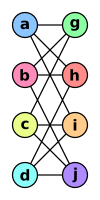
\includegraphics[width=0.2\linewidth]{image.png}} 
    \subfigure[]{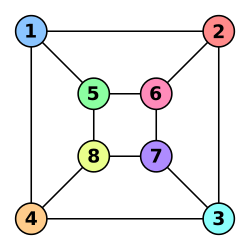
\includegraphics[width=0.4\linewidth]{image2.png}}
\end{figure}

\newpage

\subsection{Problems}
\begin{enumerate}
    \item \textbf{(Hard)} Generalize \color{red} \textbf{Problem 4.1} \color{black} from $6$ to $n$.
    \item Find the number of non-isomorphic graphs with $4$ vertices.
    \item \textbf{(Hard)} Find the number of non-isomorphic graphs with $n$ vertices.
\end{enumerate}

\section{The Lemma}

For completeness, we include the statement of the lemma here, although it will probably look like hieroglyphics.

\begin{tcolorbox}[colback=orange!5!white,colframe=orange!75!black]
  \color{orange} \textbf{Lemma 1} (Burnside.)\color{black}
  \vspace{0.1cm}
  
  Let $G$ be a group acting on a set $S$. For $\alpha \in G$, let $\text{fix}(\alpha)$ denote the set of fixed points of $\alpha$. Then\[\lvert G \rvert \cdot \lvert S/G \rvert = \sum_{\alpha \in G} \lvert \text{fix}(\alpha) \rvert .\]

  
\end{tcolorbox}
\end{document}
